
%----------------------------------------------------------------------------------------




\part{Capítulo tres}
\graphicspath{ {img/ch3/}, {img/} }

%----------------------------------------------------------------------------------------
%	CHAPTER 3
%----------------------------------------------------------------------------------------

\chapterimage{ima2} % Chapter heading image


\chapter{Aplicaciones de interés compuesto}
\section{Fórmulas del capítulo}
\begin{spacing}{1.5}
\begin{center}
\begin{tabular}{ |p{6cm}|p{7cm}| p{2cm}|}
\hline 
\rowcolor{orange!50}
\begin{center}\textbf{Fórmula} \end{center} & \begin{center} \textbf{Nombre}\end{center} & \begin{center} \textbf{Excel} \end{center} \\ \hline                       

$i =i_{1} + i_{2} + (i_{1})(  i_{2})$ & Equivalencia de tasas de referencia & - \\ \hline 

$ i_{R} = \frac{i-i_{f}}{1+i_{f}} $ &   Tasa de interés real & - \\ \hline

 
\end{tabular}
\end{center}
\end{spacing}


Muchas son las aplicaciones que tiene la fórmula de interés compuesto, aquí solo daremos algunas, las que consideramos están más de acuerdo con el plan del texto. Para empezar examinaremos los depósitos a término fijo y certificados de depósito a término.\\



\section{Depósito a término fijo}


La misión de un intermediario financiero consiste en conseguir dinero prestado generalmente del público y volverlo a prestar a otras personas, pero a una tasa más alta. Para conseguir el dinero del público debe ofrecer una tasa de interés e incentivar a los inversionistas a que le traigan sus ahorros, a esta tasa se le denomina tasa de captación. Cuando va a prestar estos dineros lo hace a una tasa mayor denominada tasa de colocación.\\

\subsection{Certificado de depósito a término}
Es el certificado que se recibe por depósitos de sumas de dinero. Los plazos pueden ser de 30 días en adelante siendo los más comunes los de 30, 60, 90, 180 y 360 días. Pueden emitirlos los bancos comerciales, corporaciones financieras y compañías de financiamiento comercial. La tasa de interés por su depósito está determinada por el monto, el plazo y las condiciones existentes en el mercado al momento de su constitución. Son nominativos y no se pueden redimir antes de su vencimiento.\\ 



\textbf{Ejemplo 1}\\

Supongamos que una persona invierte \$600.000 en un depósito a término fijo en 6 meses, si le garantizan una tasa del 24\% nominal anual mes vencido, determinar la tasa efectiva anual y el valor del documento suponiendo una retención en la fuente sobre utilidades del 7\% sobre las utilidades.\\

\begin{itemize}
	\item a. Diagrama de flujo :\\
	
	%%imagen 1
	
	\begin{center}
		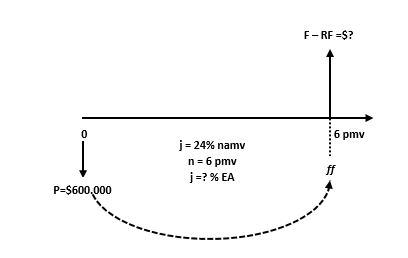
\includegraphics[height=5.0cm]{3_1}
	\end{center}
	
	\item b. Declaración de variables :\\
	F=\$?\\
	VP = \$600.000 \\	
	j a encontrar=? \%EA\\
	j dada= 24\% namv \\	
	n = 6 pmv \\
	RF= 7\% I
	
	\item c. Declaración de formulas :\\ 
	$VF=P(1+i)^n$ \hspace{35}\textit{Valor futuro dado un valor presente}\\
	j = im \hspace{35} \textit{        Tasa nominal anual}\\
	$(1+i_{1})^{m_{1}} = (1+i_{2})^{m_{2}}$\hspace{35} \textit{Equivalencia de tasas}\\
	$RF = 7\%\ I$     \textit{        Retención en la fuente} \\ 
    $I = F - P$      \textit{Monto del interés}\\ 
    $F\ neto = F - R$     \textit{         Valor futuro neto}\\
	
	\item d. Desarrollo matemático:\\
    Despejando:\\
    De la formula de equivalencia de tasas\\
    $ (1+0,02)^{12} = (1+i)^{1} $\\
    $i = (1 + 0,02)^{12} -1 = 0,26824179$\\
    $j = 0,26824179 x1 = 0,26824179 EA$\\
    $j = 26,824179\% EA$\\
    $i = 26,48\%$ pav\\
    $j = 26,48\% x1= 26,48\%\ naav = 26,48\%\ EA$\\
	VF= \$$600.000(1+0,02)^6$\\
	VF= \$675.697,45\\
	I = F - VP = \$675.697,45 - \$600.000\\
	I = F - VP = \$75.697,45\\
	RF = 0,07 x \$75.697,45 = \$5.298,82\\
	F$_{final}$ = \$675.697 - \$5.299 = \$670.398\\
	
	\item e. Respuesta:\\
	El valor del documento después de impuestos es de \$675.697,45 que es menor que F = \$675.697,45 y obviamente se reduce la tasa de nominal anual mes vencido j = 24,84\% naav .\\
	
	Observación
	\begin{itemize}
		\item La rentabilidad después de impuestos se puede calcular así:\\ \$670.398 = \$$600.000(1+i)^6$
		\item De donde se obtiene\\
		$i$ = 1,866232288 \% pmv\\
		$j$ = 1,866232288 \% x 12 = 22,3947874\% namv \\
		$(1 + i_1)^{m_1} = (1 + i_2)^{m_2}$\\
        para la EA, $m_2$\ = 1 y luego \\
        $j = i m$\\
        $j = 24,84\%\ EA,\ inferior\ al\ 26,82\%\ EA$\\
		\item Por equivalencia de tasas: 
		$i$ = 24,84\% EA (después de impuestos)\\
	\end{itemize}
	
\end{itemize}
De lo visto hasta el momento podemos concluir que si el depósito a término fijo gana el 26,84\% EA antes de impuestos, después de impuestos se reduce al 24,84\% EA, sin embargo esto no es más que una utopía porque el inversionista entregó al principio \$600.000 los cuales tenían un cierto poder adquisitivo y cuando le devuelven el dinero su poder de compra se ha disminuido por efectos de la inflación y se pregunta cuál sería la rentabilidad del depósito a término después de impuestos e inflación en términos de EA? (pendiente a retornar más adelante).\\

\subsection{Inflación (i_f)}
Mide el crecimiento del nivel general de precios de la economía. La inflación es calculada mensualmente por el DANE sobre los precios de una canasta básica de bienes y servicios de consumo para familias de ingresos medios y bajos. Con base en éstas calcula un índice denominado Índice de Precios al Consumidor (IPC). La inflación corresponde a la variación periódica de ese índice.\\
\\
Hacemos énfasis en que la inflación y la deflación son fenómenos internos a un país. (La devaluación si es un fenómeno económico externo a un país).\\


\subsection{Índice}
Es un indicador que tiene por objeto medir las variaciones de un fenómeno económico o de otro orden referido a un valor que se toma como base en un momento dado. Relación de precios, de cantidades, de valores entre dos períodos dados.

\subsection{Índice de precios al consumidor (IPC)}
Variación que entre un mes y otro presentan los precios de bienes y servicios de consumo final correspondientes a una canasta típica, donde se incluyen los servicios educativos, de salud, de alimentos y combustible, entre otros.

\subsection{Tasa promedio de captaciones Básica de Superfinanciera (TBS)}
Es la tasa promedio de captación a través de CDT y CDAT de las entidades financieras, calculada diariamente por la Superintendencia Financiera para diferentes plazos.	

\section{Devaluación (idev)}	
La pérdida de valor de una moneda frente a otra moneda se denomina devaluación, por ejemplo, habrá devaluación si inicialmente hay que pagar \$1500 por un dólar y un año más tarde hay que pagar \$2000 por el mismo dólar. En este caso la devaluación del año es igual a la variación de precio sobre el precio inicial, esto es: \\

devaluación = $\frac{\$2000-\$1500}{\$1500} = 0,333333 $ = 33,33\% pav \\

Lo contrario de la devaluación se denomina revaluación que significa que habrá que pagar menos pesos por el mismo dólar, por ejemplo, si al principio del año hay que pagar \$1500 por un dólar y al final del año hay que pagar \$1200 entonces la revaluación será variación de precio sobre el precio inicial así: \\

revaluación = $\frac{\$1200-\$1500}{\$1500} = -0,2$ = -20\% pav \\



\subsection{LIBOR (London Interbank Offer Rate)}
Tasa de interés anual vigente para los préstamos interbancarios de primera clase en Londres y Europa.\\ \\



\textbf{Ejemplo 2}\\
Un inversionista residente en Colombia adquiere un documento que vale U\$300, gana un interés del 6\% nominal anual año vencido (naav) en dólares a un plazo de un año. El tipo de cambio actual es US\$ 1 = \$1500 y se estima una devaluación del peso con respecto al dólar durante ese año del 20\% efectivo anual. Calcular la rentabilidad que se podía obtener. ¿Cuál es la rentabilidad neta, una vez descontada la retención en la fuente del 7\%?

\begin{itemize}
	\item a. Diagrama de flujo de caja:
	
	%imagen 2
	\begin{center}
		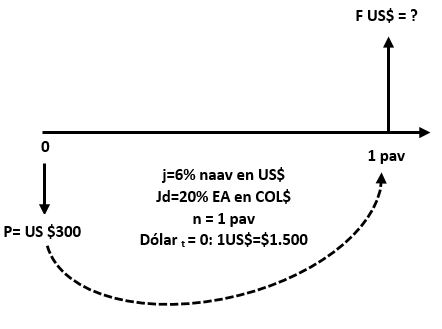
\includegraphics[height=5.0cm]{3_2}
	\end{center}
	
	
	\item b. Declaración de variables en dólares:\\
	j= 6\% naav en US$\\
    n=1 pav\\
    Dólar: 1US$=$1500\\
    j dev= 20\% EA
	
	
	\item c. Declaración de fórmulas\\        
		
		$ F = {P(1+i)^{n} $\hspace{35}\textit{ Valor futuro}\\     
	
	\item d. Desarrollo matemático:\\
	Las condiciones iniciales son: US\$300 y en pesos $300 x 1500 = \$450.000$\\
	\\ %imagen3
	
	
	
	Las condiciones finales en dólares son:\\
	$F = P(1+i)^n $\hspace{35}\textit{ Valor futuro dado un valor presente}\\
	$F = US\$300(1 + 0,06)^1 = US\$318$\\\\
	Para calcular las condiciones finales en pesos primero debemos calcular el tipo de cambio que regirá dentro de un año. \\
	
	Declaración de variables en pesos:\\
	Como la devaluación es del 20\% EA, dentro de un año un dólar valdrá\\ $VF = \$1.500(1+0,2)^ {1} = \$1.800$ y los US\$318 valdrán US\$ $318\textbf{x}\frac{\$1.800}{US\$1} = \$572.400$ tal como se aprecia en la gráfica.\\

		US$\$318 \textbf{x}\frac{\$1.800}{US\$1} = \$572.400 $ \hspace{35}\textit{ Ecuación de valor}\\

	%imagen 4
	\begin{center}
		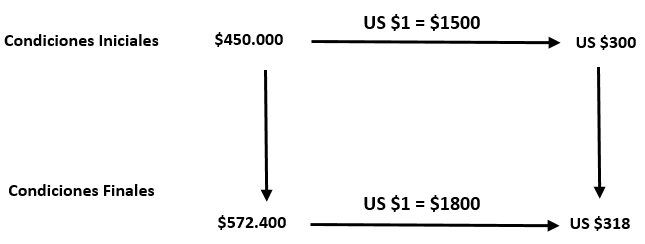
\includegraphics[height=4.0cm]{3_4}
	\end{center}
	
	
\end{itemize}
Como el inversionista reside en Colombia la rentabilidad que él necesita conocer se obtiene aplicando la fórmula del interés compuesto a los valores iniciales y finales en pesos (si el inversionista fuera residente en E.E.U.U la rentabilidad se obtendrá entre valores iniciales y finales, pero en dólares).  \\

\begin{itemize}
	\item a. Diagrama de flujo de caja:\\
	%imagen 5
	\begin{center}
		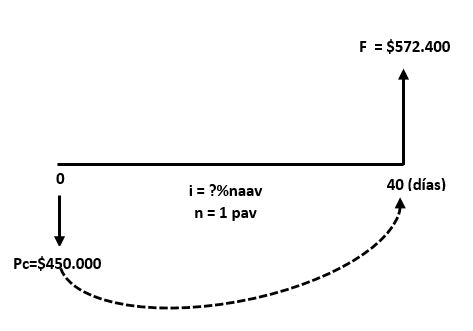
\includegraphics[height=5.0cm]{3_5}
	\end{center}
	
	\item b. Declaración de variables en pesos:\\
	Pc= \$450.000\\ F = \$572.400\\ 
	j=?\% naav\\
	n = 1 pav\\
	\item c. Declaración de fórmulas:\\
	$F = P(1+i)^n$\hspace{35} \textit{Valor futuro}\\
	\item d. Desarrollo matemático:\\
	$\$572.400 = \$450.000(1+i)^1$\hspace{35} \textit{Ecuación de valor}\\
	$i=27,2\% pav,\ \rightarrow \ j = 27,2 x1 = 27,2 \%\ EA$ \\
	$I = \$572.400 - \$450.000 = \$122.400$ \\
    $RF = 0,07 x \$122.400= \$8.568$ \\
    $F neto = \$572.400 - \$8.568 = \$563.832$ \\\\
    Aplicando la fórmula del valor futuro: \\
    $\$563.832 = \$450.000(1+i)^1$ , despejando $i = ?$ \\
    $i = 0,25296$naav \equiv  $j = 25,296\% EA$ \\
	\item e. Resultado:\\
    
    La rentabilidad que se podía obtener es 27,2\%\ EA. y la rentabilidad neta, una vez descontada la retención en la fuente del 7\%\ es 25,296 \%\ EA\\

\end{itemize}

\section{Tasas combinadas o tasas equivalentes de referencia}
En el caso anterior el inversionista ganará dos tasas, una tasa la de interés en dólares 6\% (naav) y otra la tasa de devaluación 20\% EA equivalente a 20\% (naav) (porque al final del año va a recibir más pesos por el mismo dólar).\\

Cuando se combina una tasa $i_{1}$ con una tasa $i_{2}$, con el objetivo de facilitar los cálculos se puede utilizar la tasa combinada i. Para este fin se usa la siguiente fórmula.\\
\centerline{$ i = i_{1} +i_{2} + (i_{1})( i_{2})$ \hspace{15}\textit{ Tasas combinadas}\\}
\textbf{Nota} Se utiliza únicamente para el cálculo de tasas de interés anuales\\




\textbf{Ejemplo 3}\\
Resolver el ejemplo 2 usando la tasa combinada\\

\textbf{Solución:}\\

\begin{itemize}
	\item a.Diagrama de flujo:\\
	
	%imagen 6
	\begin{center}
		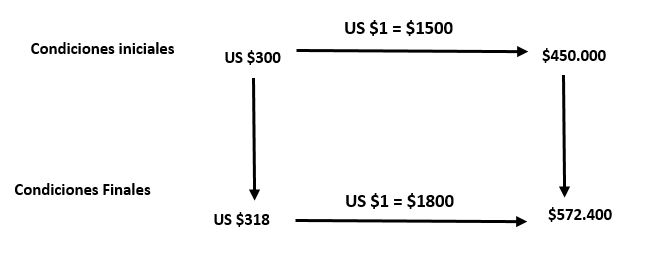
\includegraphics[height=3.5cm]{3_6}
	\end{center}
	
	
	\item b.Declaración de variables:\\
	$j_{1} = 6\%\ naav$\\
	$j_{2} = 20\%\  naav$\\
	\item c. Declaración de fórmulas:\\
	$i =i_{1} + i_{2} + i_{1}  i_{2}$\hspace{35}\textit{ Tasas combinadas}\\
	$j =i  m$\hspace{35}\textit{ Tasa nominal anual}\\
	\item d.Desarrollo matemático:\\
	$i_{1}= \frac{6 \%\ naav}{1} = 6\% $pav \\
	$i_{2}= \frac{20 \%\ naav}{1} = 20\% $pav \\
	$i= 0,06 + 0,2 + 0,06 x 0,2 = 0,272 = 27,2\% pav,\\ j = 27,2\% x1 = 27,2\ \%\ naav$ \hspace{35}\textit{ Ecuación de valor}\\
	\item e.Respuesta:\\
	Usando la tasa combinada obtenemos que el resultado es 27,2\% EA\\
	
\end{itemize}


\section{Tasa deflactada o tasa real}
Al hacer el análisis sobre proyectos de inversión es necesario tener en cuenta que la inflación afecta la rentabilidad real del proyecto y que siempre se desea obtener una rentabilidad superior a la inflación. Para calcular la rentabilidad real podemos hacer uso de la fórmula asumiendo que la inflación $i_{f} = i_ {1} $, que la rentabilidad $i_{R} = i_ {2} $ y que la rentabilidad que en total paga es i, por tanto se tiene:\\
\begin{align*}
	i= i_{f} + i_{R} + i_{f} i_{R}
\end{align*}

Despejando $i_{R}$ se tiene 
\begin{align*}
	i_{R} = \frac{i-i_{f}}{1+i_{f}}\hspace{35}\textit{ Tasa de interés real}
\end{align*}



\textbf{Ejemplo 4:}\\
Calcular la rentabilidad que gana el inversionista del ejemplo 2 teniendo en cuenta que la inflación para el año en el que se hizo la inversión fue del 18\% efectivo anual. ¿Cuál es la rentabilidad neta una vez descontada la Retención en la fuente y la inflación? \\\\

\textbf{Solución:}\\

\begin{itemize}
	\item a. Diagrama de flujo:\\
		%imagen 6
	\begin{center}
		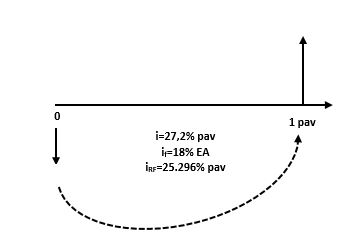
\includegraphics[height=5cm]{3_4_1}
	\end{center}
	\item b. Declaración de variables:\\
    
    $i=27,2\% pav $\\
	$i_{f} = 18\%$  EA \equiv 18\%naav \\
    $i_{f} = \frac{j}{m} = \frac{18\%}{1} = 18\%$ pav \\
    $i_{RF} = 25,296\% pav$\\ 
	\item c. Declaración de fórmulas:\\
	$ i_{R} = \frac{i-i_{f}}{1+i_{f}} $\hspace{35}\textit{ Tasa de interés real}\\
	\item d. Desarrollo matemático:\\
	
	$i_{R} = \frac{0,272-0,18}{1+0,18} = 0,077966 = 7,8\% $pav\\
	$i^{*}_{R} = \frac{(0,25296-0,18)}{(1 + 0,18)}$ \hspace{35}\textit{ Tasa de interés luego de retencion en la fuente}\\
    $i^{*}_{R} = 6,18305085\%$ pav \\
    $j^{*}_{R} = 6,18305085\%$ EA \\
	\item e. Respuesta.\\
	La rentabilidad sin descontar la retención en la fuente  fue del 7,8\% pav.\\
	\end {itemize}
	
	
	Retomando el ejemplo 3 podemos concluir que si el depósito a término fijo gana el 26,84\% EA antes de impuestos, después de impuestos se reduce al 24,84\% EA, sin embargo esto no es más que una utopía porque el inversionista entregó al principio \$600.000 los cuales tenían un cierto poder adquisitivo y cuando le devuelven el dinero su poder de compra se ha disminuido por efectos de la inflación ($i_{f}= 18\% $pav$ $) y se pregunta cuál sería la rentabilidad del depósito a término después de impuestos e inflación en términos de 7,8\%pav y una vez descontada la retención en la fuente queda en 6,18\%.\\
	
	
	\section{Combinación de tasas}
	Hay muchos créditos atados a una tasa principal, por ejemplo a la inflación más unos puntos adicionales, estos puntos adicionales se denomina el spread, suponiendo que la inflación fuera del 10\% efectivo anual y que el spread sea de 5 puntos, entonces la tasa a la cual se cancelará el crédito se puede calcular aplicando la fórmula de las tasas combinadas: \\
	
	$i= 0,1 pav + 0,05 pav + 0,1 x 0,05 = 0,155 pav \equiv 15,5\% pav $ \rightarrow  $j = 15,5\% pav x1 pav = 15,5\%naav \equiv 15,5 \%EA$ \\
	
	Cuando la tasa principal viene dada en forma efectivo anual para agregarle el spread se usa la fórmula de combinación de tasas, pero si el spread se le adiciona a una tasa nominal entonces el spread simplemente se suma a la tasa principal, por ejemplo: \\
	
	Si un préstamo para vivienda se otorga a la tasa de los depósitos a término fijo-DTF (tasa principal) más 8 puntos y suponiendo que la tasa de depósito a término fijo -DTF lo mismo que la sea del 17\% nominal anual trimestre anticipado, entonces la tasa del crédito será: \\
	
	$i = i_{1} + i_{2}
i = 17\%nata + 8\%nata = 25\% nata$\\\\ Las tasas equivalente nominales se suma en igual periodo y modalidad, en tasas efectivas anuales se aplica la equivalencia de tasas de referencia.\\
	
	Por equivalencia de tasas se concluye que es equivalente al 29,45\% efectivo anual.\\
	
	\textbf{Observación:} Para créditos es costumbre que la tasa de depósito a término fijo -DTF lo mismo que la tasa de captación de las corporaciones-TCC se expresan en nominal anual trimestre anticipado y en tasa de captación de la tasa de depósito a término fijo -DTF y de la tasa de captación de las corporaciones-TCC se expresa en efectivo anual.\\
	
	
	
	\textbf{Ejemplo 5}\\
	
	Supongamos que una persona tiene un préstamo hipotecario al IPC + 4 puntos ¿Cuál debe ser el spread si se cambia a otro plan cuya tasa es la DTF +X? Suponga que el IPC = 8\% efectiva anual y que la DTF = 18,67\% nominal anual trimestre vencido, en donde
IPC: Tasa del Índice de Precios al Consumidor
DTF: Tasa de Depósito a Término Fijo promedio \\
	
	\textbf{Solución:}\
	\\
	
	\begin{itemize}
		\item a. Diagrama de flujo\\
		No se Requiere \\
		\item b. Declaración de variables\\\\
		$j_{1}= 8\% EA \\ j_{2} = 18,67\% nata$\\
		\item c.Declaración de fórmulas:\\\\
		IPC + 4 = DTF + X  Ecuación de valor\\
		ECUACION DE EQUIVALENCIA \\
        
        Tasa del crédito = IPC + 4 puntos efectivos anuales = DTF + X (spread en \% nata) \\
        $i = i_1 + i_2 +i_1 * i_2$ \\
		$i_{a}= \frac{i}{1+i}$\\
		$(1 + i_{1})^{m_{1}} = (1 +i_{2})^{m_{2}}$\\
		$j_{a} = i m$\\
		\item d. Desarrollo matemático:\\\\
		IPC+4 = 0,08 + 0,04 + 0,08 x0,04\\
		Tasa del crédito = IPC + 4 puntos\\
        Tasa de crédito inicial= 0,08 + 0,04 + 0,08x0,04 EA\\
		IPC+4 = 12,32\% pav equivalente a 12,32\% EA \\
		$(1 + 0,1232)^1 = (1 + i) ^4$ Fórmula de equivalencia de tasas para convertir la tasa de crédito del 12,32\% EA a una periódica trimestre vencido y a su vez a la tasa nominal anual trimestre anticipada.\\
		i= 2,947137112\% ptv\\
		
		$i_{a}= \frac{0,02947137112}{1+0,02947137112} = 0,0286275\%$ pta\\
		$j_{a} = 2,86875\% * 4 = 11,451\%$ nata\\
		
		Tasa de crédito equivalente= DTF + 4 (\%nata) \\
        Tasa de crédito equivalente = 11,45 \% nata = 18,67\% nata + X \%nata \\
        Entonces X = 11,451\% nata - 12,32\% nata = -7,219\% nata \\
		DTF + X = 0,1867 + X nata \\
		0,11451 = 0,1867 + X; de donde X = -0,07219 \\
		X = -7,219\% nata\\
		
		\item e. Respuesta\\
		
		Finalmente podemos concluir que si se cambia de plan tendrá que ser la DTF menos 	7,219\%	nata\\
		
	\end{itemize}
	
	\textbf{Observación 1:}En Colombia el spread se da en puntos que son adicionales a la tasa principal, en Europa y Estados Unidos el spread se acostumbra a dar en puntos básicos. Un punto básico es igual al 0,01\% de forma que 400 puntos básicos corresponden a un spread de 4 puntos.\\
	
	\textbf{Observación 2:}A pesar de que la Libor es una tasa efectiva, es costumbre que el spread simplemente se sume a la Libor sin hacer uso de la tasa combinada, La razón es que éstas tasas son muy pequeñas y la diferencia de resultados entre un método y otro es prácticamente nula.\\
	
	\textbf{Ejemplo 8}\\
	Una industria tiene actualmente contratado un préstamo con una corporación financiera a la tasa del TCC+3 puntos. ¿Cuál debe ser el spread en puntos básicos de forma tal que financieramente sea indiferente el préstamo en la corporación financiera o en el mercado de Londres? Suponga los siguientes índices: \\
	
	TCC = 15,3 \% nata \\
    $i_{dev}$ = 22\% EA. Interés devaluación del peso Colombiano con respecto a la libra esterlina. \\
    Libor = 5,2\% EA. Tasa de interés del mercado europeo \\
	
	Solución:
	\begin{itemize}
		\item a. Diagrama de flujo:\\
		No se requiere
		\item b. Declaración de variables:\\
		
		TCC = 15,3\% nata\\
		$i_{dev} = 22\%$ EA\\
		Libor = 5,2\% EA\\
		\item c. Declaración de formulas:\\
		
		$i_{dev} + Libor + X = TCC + 3$  Ecuación de valor\\
		\item d. Desarrollo matemático:\\
		
		TCC + 3 puntos= 15,3\%nata + 3\%nata = 18,3\%nata\\
		j crédito = TCC + 3 puntos nata = 15,3\% nata + 3\% nata = 18,3\% nata, tasas nominales sumas los dígitos. En tasas efectiva anual aplicamos la formula de las tasas combinadas: $i = i_{1} + i_{2} + i_{1} i_{2}$ \hspace{35}\textit{  Equivalencia de tasas de referencia} \\
        
        $j_{c} = 18,3\% nata$ \\
        $j_{c} = ?$ EA en Londres \\
		
		18,3\%npta ~ 20,601\% EA . A partir de las del crédito en TCC, 18,3\% nata, calculamos la tasa Anual Efectiva equivalente, encontrando la tasa periódica ($j = i*m$)
        y a partir de la tasa periódica anticipada llegamos a la tasa periódica vencida ($i_{a} = \frac{i}{(1+i)}$).\\
        Teniendo la tasa periódica vencida utilizamos la formula de las tasas equivalentes:
        $(1 + i_{1})^{m_{1}} = (1 + i_{2})^{m_{2}}$, en donde $m_{1}$ es igual 1, periodo anual vencido de liquidación de la tasa EA.\\
		$i_{dev} + Libor + X = 22\% + (5,2+ X)\%$\\
		crédito equivalente = 22\% EA + (libor + X) \%\ EA = ? \% EA, por la fórmula de combinación de tasas, por ser tasas EA.\\
		0,28344 + 0,0122 + X = 0,20601. (Despejar la X) \\
		X = -6,35\% \\
		\item e. Respuesta:\\
		
		Lo que significa que cobrar TCC + 3 puntos es lo mismos que cobrar devaluación más Libor menos 6,35 puntos\\
	\end{itemize}
	
	
	\section{Aceptaciones bancarias y financieras}
	\textbf{Ver link} https://prezi.com/ewsfyuf6vepz/aceptaciones-bancarias/\\
	
	Las aceptaciones bancarias y financieras son letras de cambio con cargo a un comprador de bienes manufacturados que una entidad financiera avala o garantiza su pago al poseedor de la aceptación de vencimiento. El plazo máximo es de un año. Cuando la entidad financiera que da el aval es un banco se denomina aceptación bancaria, si es otro tipo de entidad financiera se denomina aceptación financiera.\\
	
	Las aceptaciones en general son títulos que se expiden a la orden del proveedor, no son divisibles, no son gravables en el mercado primario.\\
	
	\textbf{Ejemplo 9}\\
	Supongamos que un proveedor de bicicletas (puede ser la fábrica) recibe un pedido de compra de 50 unidades para un almacén por valor de \$ 5 millones, pero el almacén pide un plazo de 90 días para pagar. El proveedor acepta el pedido, pero solicita que una entidad financiera garantice el pago futuro, por tal motivo el dueño del almacén se dirige a su banco y le solicita que expida una aceptación bancaria por \$ 5 millones con vencimiento en 90 días, el banco le entrega al almacén la aceptación y éste se la entrega al proveedor, este último puede guardar la aceptación y cobrarla al banco a su vencimiento o puede negociarla en el mercado secundario.\\
	
	%imagen ejemplo 9
	\begin{center}
		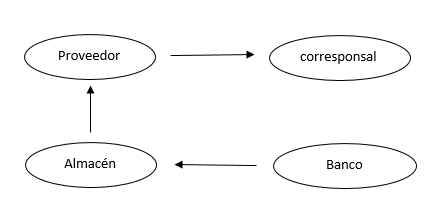
\includegraphics[height=4.0cm]{3_7}
	\end{center}	
	
	Puede ocurrir que el fabricante se encuentre en un país distinto al del almacén y si el banco no tiene sucursal en ese otro país deberá tener corresponsales (es decir bancos que lo representen en ese otro país). Si el proveedor necesita el dinero antes del vencimiento, puede ofrecer en venta la aceptación y para ello tiene dos opciones: Venderla al mercado extra bursátil, que tiene la ventaja de no pagar comisiones a intermediarios porque se negocia en forma directa o venderla al mercado bursátil, es decir en una bolsa de valores, a través de un intermediario de bolsa conocido como corredor de bolsa que cobra una comisión por sus servicios de intermediación.\\
	
	Es obvio que, al vencimiento de la aceptación, el dueño del almacén deberá cancelar al banco el valor de ésta e independientemente de si el almacén le paga o no al banco la aceptación, el banco sí tendrá que pagar en la fecha de vencimiento el valor nominal de la aceptación al tenedor de ésta. A continuación, presentamos una gráfica más completa donde se muestra la trayectoria de la aceptación bancaria.\\
	
	%imagen ejemplo 9_2
	\begin{center}
		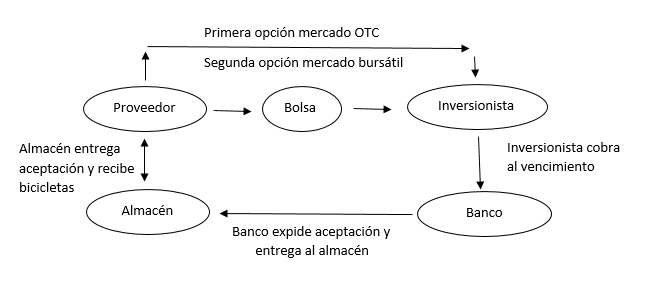
\includegraphics[height=5.0cm]{3_8}
	\end{center}	
	
	\textbf{Primera opción}: Supongamos que faltando 40 días para el vencimiento, el proveedor debido a un estado de iliquidez, decide vender la aceptación en el mercado extra bursátil, (el inversionista que adquiere esta aceptación puede ser un particular, una compañía de financiamiento comercial, una leasing, etc.) Supongamos que la tasa convenida es del 30\% periódico año vencido es diferente a una tasa de descuento del 30\% del valor final = d. Tomar el año de 365 días.\\
	Es costumbre calcular el Pc como un porcentaje del valor que tendrá la aceptación al vencimiento. (El valor al vencimiento se denomina valor de maduración o valor de redención y lo representaremos por F).
	Haciendo el cálculo por cada \$ 100 de valor de maduración se tendrá: \\\\\\\\\\\\\\
	
	\begin{itemize}
		\item a.Diagrama de flujo\\
		\begin{center}
			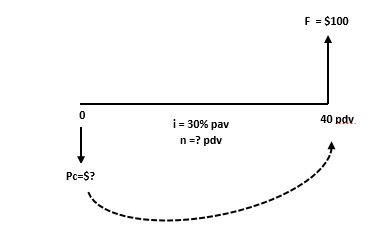
\includegraphics[height=5.0cm]{3_9}
		\end{center}	
		\item b. Declaración de variables\\
		
		P = \$? \\
		VF = \$100\\
		i=30\% pav\\
		$n = \frac{40}{365}$ pav	       
		\item c. Declaración de formulas:\\
		
		F =  $P(1+i)^n$ \hspace{35}\textit{Valor futuro}\\
		\item d. Desarrollo matemático:\\
		
		VP = $\$100(1+0,3)^\frac{-40}{365}$ = \$97,1657\\
		Pc=\$5.000 x 97,1657\% = \$4.858,285\hspace{35}\textit{Ecuación de valor}\\
		Entonces si el precio de compra Pc es de \$97,1657 el precio de compra para una aceptación de 100 pesos el precio de compra para \$5000 es 5000x (0,971657).\\
		
		\item e. Respuesta\\
		El valor que se invirtió fue \$4.858,285\\
	\end{itemize}
	
	\textbf{Segunda opción:} El proveedor decide descontar la aceptación en el mercado bursátil y en tal caso debe recurrir a un corredor de bolsa (quienes son los únicos autorizados para negociar en la bolsa) y supongamos que el corredor le dice que en la bolsa este tipo de operaciones se está registrando al 30\% periódica 40 días vencido, esta tasa se denomina tasa de registro porque es la tasa que queda registrada en las computadoras de la Bolsa y la representamos por $i_{R}$. Con base en la tasa de registro se puede calcular el precio de registro así: \\
	$P_{v}= \$100  (1 + 0,35)^{\frac{-40}{365}}$ Equivalente al 97.1657 \$.\\
	El precio de este registro en pesos será: 97,1657\$ x \$5'000.000 = \$4.858.285\\
	De esta forma en las computadoras de la Bolsa va a aparecer en venta esta aceptación por valor de 97.1657\% de su valor nominal de registro y que a ese precio produce una rentabilidad del 30\% periódica 40 días vencidos.\\
	Pero además el corredor le dice que para que la aceptación sea inscrita en bolsa tendrá que pagar una comisión que representaremos como COMv (Comisión de venta).\\
	Supongamos que la comisión de venta sea del 0,5\% en rentabilidad entonces la tasa total de descuento será: \\
	$i_{R} + COMv = 30\% + 0,5\% = 30,5\%$ p(40d)v\\
	Esta nueva tasa se denomina tasa de cesión o tasa del vendedor.\\
	Con base en la tasa de cesión podemos calcular el valor de cesión o sea el valor que recibe el vendedor para la aceptación. El precio de cesión lo representaremos por Pv (precio de venta), \\
	$P_{v}  = \$100(1+0,35)^\frac{-40}{365} = \$97,1248 $ equivalente a 97.1248\%\\
	$P_{v} = 97.1248 < P_{R} = 97.165$\ porque está cediendo un valor al comisionista vendedor.\\
	El precio de venta en pesos o precio de cesión en pesos será: 5.000.000 \text{x} 0,971248 = \$4.856,240\\
	
	\textbf{Observación:} El valor de la comisión de venta se puede hallar por la diferencia entre los precios de venta y el precio de registro esto es: \\
	COMv= 4.858.285 - 4.856.240 = \$2.405\\
	
	\textbf{Ejemplo 10}\\
	
	Supongamos que un inversionista desea adquirir la aceptación bancaria del ejemplo anterior la cual figura con una tasa de registro del 30\% periódico 40 días vencido y con precio de registro P_{R} = 97,165\% pero él también sabe que para adquirirla deberá pagar una comisión a un corredor de bolsa lo cual hará variar el precio que él debe pagar y también la rentabilidad que él pueda obtener.\\
	
	Supongamos que la comisión que cobra un corredor por la compra es del 0,475\% periodo 40 días periodo vencido\\
	¿Cuál es el precio del inversionista? $P_{c} = \$$?, que incluye la comisión de bolsa de comprador, el precio de registro y la comisión del comisionista vendedor. El punto de referencia es el precio de registro P_{R}.\\
	¿Cuál es la rentabilidad del inversionista? $i_{c} =? \%$ periódica 40 días vencido, o $j =? nadv$\\
	
	\textbf{Solución}\\
	\begin{itemize}
		\item a. Diagrama de flujo\\
		\begin{center}
			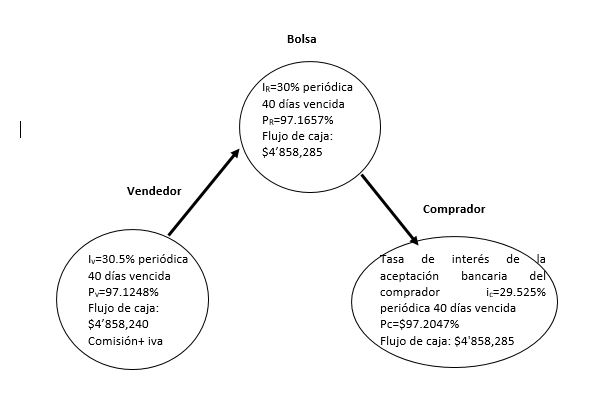
\includegraphics[height=8.0cm]{3_10}
		\end{center}	
		\item b. Declaración de variables\\ 
		$i_{c} = 30\% - 0,475\% = 29,525\% p(40dv)\\
		VPc = ?\\
		$n= -\frac{40}{365}\\$\\
		P_{R}=?$\\
		\item c.Declaración de formulas\\
		P = $F(1+i)^{-n}$ \hspace{35}\textit{Valor presente}\\
		\item d. Desarrollo matemático:\\
		Pc = $ \$100(1+0,29525)^\frac{-40}{365} = \$97.2047$ \hspace{35}\textit{Ecuación de valor} \\
		$P_{R}$ = \$97.2047\% x \$5.000.000 = \$4.860,245\\
		Pc-$P_{R}$ = \$4.860,235 - \$4.858,285 = \$1.950\\ 
		\item e. Respuesta\\
		Precio del Inversionista = \$ 97.2047 y la rentabilidad inversionista fue de 29,52\% P= 40 dv \\

		
	\end{itemize}
	\textbf{Observación:} En el mercado bursátil el precio del vendedor es diferente al precio del comprador debido a la comisión de los corredores de bolsa, pero en el mercado extrabursátil estos valores son iguales dado que no hay comisión.\\
	
	En el ejemplo anterior hemos mostrado el procedimiento de negociación en los mercados extra bursátil y bursátil, pero por simplicidad no hemos incluido el impuesto y la comisión que cobra el banco por la expedición de la aceptación bancaria. En el siguiente ejemplo incluiremos este factor.\\
	
	\textbf{Ejemplo 11}\\
	El dueño del almacén solicita al banco una aceptación bancaria por \$5 millones, que entregará al proveedor (fabricante) para que le entreguen la mercancía; para que el banco preste este servicio le cobra al dueño del almacén una comisión que puede ser del 1\% por mes pagadero en forma anticipada sobre el valor de la aceptación, esto es 1\% x 5.000.000 = \$50.000 por cada mes y por los 3 meses que dura la aceptación será: \$50.000 x 3 = \$150.000, además habrá que pagar otra carga impositiva que es el IVA, que en el momento es del 16\%, así que en pesos el IVA será: 16\% x \$150.000 = \$24.000 de manera que el costo total de apertura de la aceptación bancaria para el dueño del almacén viene a ser \$150.000 + \$24.000 = \$174.000. El $P_{R}$ = \$4.860,245 del ejemplo anterior.\\
	¿Cuál es el precio de aceptación? \\
	¿Cuál es la rentabilidad? \\
	
	\begin{itemize}
		\item a. Diagrama de flujo\\
		\begin{center}
			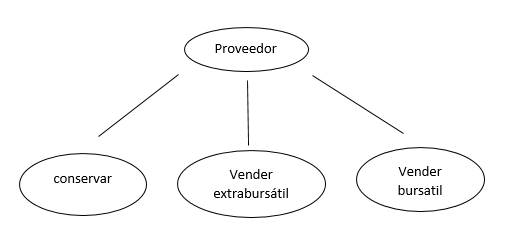
\includegraphics[height=4.0cm]{3_11}
		\end{center}	
		\item b.Declaración de variables\\
		rf=7\% de las utilidades\\
		VF = \$5.000.000\\
		$VP_{R}$ = \$4.858,285\\
		\item c. Declaración de formulas\\
		RF = rf * (F - $P_{R}$) \\
		\item d. Desarrollo matemático\\
		
		Si la aceptación es vendida en el mercado bursátil, ya no habrá IVA (puesto que ya fue pagado en el momento de la apertura de la aceptación) pero en cambio habrá otra carga impositiva que grava las utilidades sobre activos financieros denominada retención en la fuente la cual representaremos RF cuya tarifa actual (1999) es del 7\%, de las utilidades, es decir que se aplica a la diferencia entre el valor de redención y el precio del registro.\\
		Si la aceptación es vendida en el mercado bursátil 40 días antes del vencimiento a un inversionista, según el ejemplo 10, el precio de registro es \$4858,258, en consecuencia, la retención en la fuente la podemos calcular así: \\
		\begin{center}
			RF = 0,07(\$5.000.000 - \$4,858,258) = \$ 9,920\\
		\end{center}
		
		\item e. Respuesta:\\
		\begin{center}
			RF = \$9920
		\end{center}
		En consecuencia, el comprador (que viene a ser el inversionista) deberá pagar el precio de compra más la retención en la fuente lo cual viene a dar: \\
		\begin{center}
		    $Pc = \$4.860,235 + \$9.920 = \$4.870,155$
		\end{center}
		
	\end{itemize}
	\textbf{Observación 1:}La nueva $i_{c}$ se reduce al 27,137419\% periódica 40 días vencido con respecto a la $i_{R}$ del 30\% periódica 40 días vencido, e incluye la comisión bursátil y la retención en la fuente (por la totalidad de rendimientos en 90 días).\\
	
	\textbf{Observación 2:} El $i_{v}$ se aumenta X\%EA con respecto al $i_{R}$ del 30\% EA, incluye la comisión bursátil del vendedor, comisión de expedición de la aceptación bancaria e IVA:\\
	\\
	\\
	\\
	\\
	\textbf{Tabla de rentabilidad en anual efectivo}\\
	
	\textbf{Ejercicio 12}\\
	
	Supongamos que faltando 10 días para el vencimiento el inversionista del ejemplo anterior decide venderlo y para esta época se están negociando en Bolsa con una tasa del 28\% período 10 días vencido, por lo tanto la tasa de registro debe ser del 28\% período 10 días Vencido y el precio de registro será: \\
	\begin{itemize}
		\item a.Diagrama de flujo:\\
		
		\item b.Declaración de variables

			Pr = \$?\\ F = \$100\\ i= 28\% p(10d)v \\$n= \frac{10}{365}$p(10d)v\\

		\item d.Declaración de formulas:\
		
			$P=F(1+i    )^{-n}$\hspace{35}\textit{Valor presente}\\
		
		\item e. Desarrollo matemático
	
			$P_{R}=\$100 (1+0,28)^\frac{-10}{365}$ = 99,32595\% \hspace{35}\textit{Ecuación de valor}\\
	
		En pesos el precio de registro será: 99,3595\% x \$5.000.000 = \$4.966,298\\
		Por lo tanto, la retención en la fuente será RF = 0,07*(\$5.000.000 - \$4.966,298) = \$2.359\\
		Suponiendo que las comisiones de compra y venta sean c/u del 0,5\% en rentabilidad la tasa del vendedor viene a ser 28\% + 0,5\% = 28,5\% período 10 días vencido y el precio de venta será:
		\begin{center}
		$	P_{V} = 100(1+0,285)^\frac{-10}{365}$ = 99,3153\% equivalente a 99.3153\% * \$5.000.000 = \$4.965,765\\
		\end{center}
		Por lo tanto el vendedor además de recibir los \$4.965.765 también debe recibir lo correspondiente a la retención en la fuente (\$2,359), En consecuencia el vendedor recibirá:\\
		\begin{center}
		$P_{V}$ = \$4.966.830 + \$2.539 = \$4.969.189
		\end{center}
		Para el comprador se tiene:
		\begin{center}
			Tasa de compra ic = 28\% - 0,5\% = 27,5\% p10dv
		\end{center}
		Precio de compra:
		\begin{center}
			Pc = $100(1+0,275)^\frac{-10}{365}$ = 99,3366\% equivalente a 99,3366\%*\$5.000.000 = \$4.966.830
		\end{center}
		El total que debe pagar el comprador será el precio de compra más la parte de retención en la fuente que la Bolsa le devuelve al vendedor, esto es:
		\begin{center}
		VPc Neto= 	\$4.966.830 + \$2.359 = \$4.969.189
		\end{center}
		\item e. Respuesta\\
		\textbf{Observación 1:} El primer inversionista pagó por retención en la fuente \$9.920 y le reintegraron \$2.359 esto significa que en total pagó: \$9.920-\$2.359	= \$7.561 y el segundo inversionista pagó \$2.359\\
		\textbf{Observación 2:} La constitución de aceptaciones no implica desembolsos de dinero en forma inmediata ni por parte de la entidad financiera ni por parte del comprador, salvo el IVA y la comisión de intermediario financiero, lo demás es una obligación futura.\\
		\textbf{Observación 3:} Si una aceptación no es cobrada al vencimiento, el emisor debe consignar el valor de esta en el Banco Agrario, sin embargo el emisor da un período de gracia antes de hacer la correspondiente consignación.
	\end{itemize}
	\medskip
	
	\textbf{Ejemplo 13}\\
	
	Una aceptación bancaria por \$80 millones con fecha de vencimiento el 17 de diciembre de 1999 es adquirida en 22 de julio de 1999 por un primer inversionista con un descuento de 28\% período 28 días vencidos y es cedida a un segundo inversionista el 14 de octubre de 1999. Si el segundo inversionista desea ganarse el 32\% período días vencido, utilice un interés comercial (año de 360 días) \\
	¿Cuál es la ganancia en pesos del primer inversionista? \\
	¿cuál es la rentabilidad periódica días vencido del primer inversionista? \\
	
	Si tomamos en cuenta que debemos usar un año de 360 días entonces los días que hay entre el 22 de julio y el 17 de diciembre son 145 que se calculan así: \\
	
	\begin{center}
		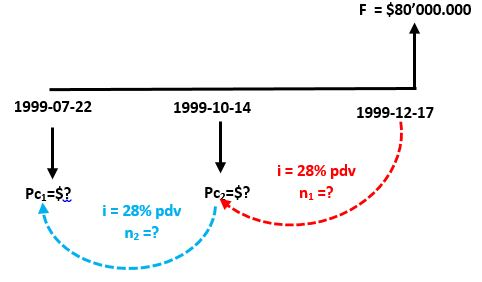
\includegraphics[height=5.0cm]{3_12}
	\end{center}
	
	Los días que hay entre el 14 de octubre y el 17 de diciembre se calculan así:
	

	\begin{center}
		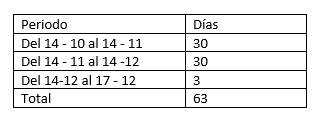
\includegraphics[height=3.0cm]{3_13}
	\end{center}
	
	\textbf{Solución}\\
	\begin{itemize}
		\item a. Diagrama de flujo\\
		\begin{center}
			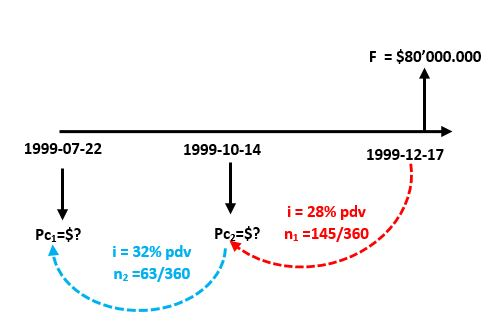
\includegraphics[height=4.0cm]{3_14}
		\end{center}
		\item b. Declaración de variables\\
		$i_{1} = 28\% pav$ \\
		$n_{1} = \frac{145}{360}$ pav\\
		$i_{2} = 32 \% pdv$\\
		$n_{2} =\frac{63}{360}$pdv\\ 
		 $n_{3} = 145$ días - 63 días = 82 pdv.\\

			$P_{c2}-P_{c1} = ?$\\\\

		\item c. Declaración de formulas\\
		
			P = $F(1+i)^{-n}$ \hspace{35}\textit{Valor presente}\\
		
		\item d. Desarrollo matemático\\
		$Pc_1 = \$80.000.000(1+0,28)\frac{-145}{360}$ = \$ 72.428.283,64 \simeq \$72.428.284 \hspace{35}\textit{Ecuación de valor}\\
		$Pc_2 = \$80.000.000(1+0,32)\frac{-63}{360}$ = \$ 76.206.067,12\\ 
		\item e. Respuesta:\\
		La ganancia del primer inversionista será:\\
		\begin{center}
			$Pc_2 - Pc_1 = \$76.206.067 - \$72.428.284 = \$3.777.783$\\
		\end{center}
	\end{itemize}
	En este caso el tiempo se puede hallar calculando los días que hay entre el 22 de julio y el 14 de octubre usando el procedimiento anterior, o, también por diferencia de días entre el total que es 145 y los que hay entre la fecha de compra del segundo inversionista y a la fecha de vencimiento que vienen a ser 63 días, entonces esta diferencia viene a ser: 145 - 63 = 82
	\begin{center}
		\$76.206.067 = $\$72.428.284(1+i)\frac{82}{360}$
	\end{center}
	De donde se obtiene que i= 25,01\%\ período 82 días vencidos \\
	La rentabilidad del segundo inversionista obviamente es del 32\% periodo (63 días vencidos).

	
	
	
	
	
	
	
	
	%\chapter{Modelos de Conteo}
	
	%\section{Introducción}\index{Introducción}
	
	
	
	%----------------------------------------------------------------------------------------
	%	PART
	%----------------------------------------------------------------------------------------
	
	%\part{Parte Dos}
	
	%----------------------------------------------------------------------------------------
	%	CHAPTER 3
	%----------------------------------------------------------------------------------------
	
	%\chapterimage{ima2} % Chapter heading image
	
	
	%Anexos
	%\chapter*{Anexos}
	%\addcontentsline{toc}{chapter}{\textcolor{ocre}{Anexos}}
	
	
	
	
	%----------------
	
	%----------------------------------------------------------------------------------------
	%	BIBLIOGRAPHY
	%----------------------------------------------------------------------------------------
	
	%\chapter*{Bibliografía}
	%\addcontentsline{toc}{chapter}{\textcolor{ocre}{Bibliografía}}
	%\section*{Books}
	%\addcontentsline{toc}{section}{Books}
	%\printbibliography[heading=bibempty,type=book]
	
	%\begin{itemize}
	%\item
	
	
	%\end{itemize}
	
	
	%----------------------------------------------------------------------------------------
	%	INDEX
	%----------------------------------------------------------------------------------------
	
	\cleardoublepage
	\phantomsection
	\setlength{\columnsep}{0.75cm}
	\printindex



